\documentclass[12pt]{extarticle}
\usepackage{amsmath, amsthm, latexsym, tikz, graphicx, listings, microtype, mathtools, soul, color, fancyhdr, amssymb}
\usepackage[margin=1in]{geometry}
\usepackage{setspace}

\newenvironment{myindentpar}[1]%
 {\begin{list}{}%
         {\setlength{\leftmargin}{#1}}%
         \item[]%
 }
 {\end{list}}
 
\DeclarePairedDelimiter\abs{\lvert}{\rvert}%
\DeclarePairedDelimiter\norm{\lVert}{\rVert}%

% Swap the definition of \abs* and \norm*, so that \abs
% and \norm resizes the size of the brackets, and the 
% starred version does not.
\makeatletter
\let\oldabs\abs
\def\abs{\@ifstar{\oldabs}{\oldabs*}}
%
\let\oldnorm\norm
\def\norm{\@ifstar{\oldnorm}{\oldnorm*}}
\makeatother

\definecolor{lightgray}{gray}{0.65}
\definecolor{pinegreen}{RGB}{1, 171, 161}
\definecolor{lightblue}{RGB}{135, 206, 250}
\definecolor{dkgreen}{rgb}{0,0.6,0}
\definecolor{gray}{rgb}{0.5,0.5,0.5}
\definecolor{mauve}{rgb}{0.58,0,0.82}
\definecolor{darkblue}{rgb}{0.0,0.0,0.6}
\definecolor{cyan}{rgb}{0.0,0.6,0.6}

\newcommand*{\Value}{\frac{1}{2}x^2}%
\newcommand{\hlc}[2][yellow]{ {\sethlcolor{#1} \hl{#2}} }

\lstset{frame=tb,
  language=SQL,
  breaklines=true,
  showstringspaces=false,
  columns=flexible,
  numbers=none,
  tabsize=3,
  escapeinside={(*@}{@*)}
  %,
  %commentstyle=\color{dkgreen},
  %stringstyle=\color{mauve}
}
\pagestyle{fancy}
\fancyhf{}
\renewcommand{\headrulewidth}{0pt}
\rfoot{\thepage}
\pagenumbering{arabic}

\definecolor{codegray}{gray}{0.9}
\newcommand{\code}[1]{\colorbox{codegray}{\texttt{#1}}}

\begin{document}


\pagenumbering{gobble}
\vspace*{15mm}
\begin{center}
{\huge
QUAC - Quick Unmanned Air Courier\\[.5ex]}
\ \\
{\LARGE 
Project Proposal\\}
\ \\
\ \\

\includegraphics[scale=0.8]{logo.png}

{\LARGE
Andrew Kirfman\\[.5ex]
Diego Oliveros\\[.5ex]
Regan Vecera\\[.5ex]
Sam Gwidyr\\[.5ex]}

\ \\
\ \\
\ \\

{\LARGE 
Department of Computer Science \\
Texas A\&M University \\
\ \\
\ \\
September $22^{nd}$}
\end{center}
\newpage
\pagenumbering{arabic}

\setcounter{tocdepth}{3}
\tableofcontents

\newpage
\section{Executive Summary}

There is currently a high demand for delivery services. However, existing solutions are often expensive, detrimental to the environment, require a substantial amount of effort for both the customers and the providers, and are slow for customer standards. The Quick Unmanned Air Courier project intends to create a delivery service which can outclass all others by delivering packages swiftly and at an affordable price.

The Quick Unmanned Air Courier involves an unmanned aerial vehicle which will be capable of delivering a package between two geographic locations. Another component is an online web interface which can communicate with the drone. Using the online web interface, the user will be able to send coordinates to the drone indicating the starting location and destination. Using this information, the drone will promptly fly to the starting location and await for a package to be loaded. After the drone has been successfully loaded, it will deliver the package to the destination coordinates.

A PixHawk flight control system will be used to manage most electrical components. This includes a GPS module to allow for a sense of direction and to transmit the drone’s location to the user. The PixHawk will also control four rotary blades through the use of four motors. The four motors and the flight controller will be powered by a 5200mAh battery using an electronic speed controller.

The drone will contain a custom made frame with a mounting point for a cargo compartment. A button will be visibly placed in this frame to allow user to notify the drone when a package has been loaded. The cargo compartment will be big enough to house a large novel. A 3D printed shell will be made to house all the electrical components within the drone’s frame to protect it from natural sources.

The drone will be able to carry packages weighing up to 3 lbs. It will fly at a height which allows it to go over most obstacles while complying with FAA regulations. It will also land safely if low on power or if affected by a mechanical malfunction.

This project intends to make the customer experience as effortless as possible. The user needs only to provide the starting coordinates and the delivery location. The online web interface will be fully interactive. It will display the real-time location of the drone while in flight. The user may also change the package’s delivery point by altering the destination coordinates.

We expect this project to revolutionize delivery services by allowing companies to offer an automated intra-day delivery service which is inexpensive, straightforward to use and reliable. This project will also benefit customers by allowing them to consume a service which is considerably better than any other alternatives.

\section{Introduction}

The Quick Unmanned Air Courier project seeks to address many troublesome issues and inefficiencies currently inherent in traditional shipping services.  These problems include, but are not limited to: being bound to road traffic and fluctuations thereof, employing costly human drivers, and being obligated to allocate money for fuel consumption.  The overall goal of our project is to use off-the-shelf, easily available parts to construct a drone capable of delivering packages between two geographic locations.  Deliveries will be easily schedulable on any web capable device through a convenient online interface.  This portal will also serve as a scheduling program for active delivery drones.  The online web interface will also be capable of changing the destination of a package mid-flight, and it will be able to display in-flight updates and statistics to users in real time.  Ultimately, the drone and associated server system must be more efficient, more conscious of the environment, and require considerably less money to operate than current comparable logistic networks such as those implemented by UPS and FedEx.  

\ \\
The project epitomizes the tenants of computer engineering by requiring equally complex hardware and software systems.  Constructing the drone hardware will require the custom setup of an entire flight control system as well as rapid prototyping to form a frame and a cargo compartment.  The software will require a fully functional and feature rich web interface, an efficient scheduling algorithm, and custom application software so that the server can communicate with the drone(s) over a network. 

\subsection{Needs Statement}

There is currently high demand for a service which can deliver online orders quickly, cheaply, and effortlessly to consumers.  Existing solutions which attempt to address this need incur too high of a cost to consumers and distributors, have a detrimental impact on the environment, require an excessive amount of human labor, and are slow by most impatient consumers' standards. 


\subsection{Goals \& Objectives}

The primary aspiration of this project is to design and implement a system consisting of an unmanned aerial vehicle, and a user interface capable of transporting small packages between any two geographic locations.  

\ \\
The objectives that we considered and the constraints that we faced when designing this system are as follows:

\begin{itemize}
    \setlength\itemsep{-0.1em}

    \item In order to be affordable for small companies with limited finances, the drone itself must incur a cost of less than \$600.
    \item To be able to transport a wide variety of small packages, the drone must be able to handle payloads which weigh up to 3 lbs and or are approximately the size of a large novel.
    \item The drone must be able to effectively fly at a height which allows it to go over most obstacles while still complying with FAA regulations regarding UAV operation.
    \item The drone must receive instructions from a central server which dictate its starting and ending locations.
    \item The drone must be capable of changing its destination mid-flight via user input from a convenient online web interface.
    \item The drone must send its location to an online web interface, allowing any user to check the status of his or her packages.
    \item The drone must land safely if low on power or afflicted by some other mechanical malfunction.

\end{itemize}
\par

\subsection{Design Constraints \& Feasibility}

\ \\
Our intra-day delivery UAV faces many limitations and considerations that must be factored in to our design process.  Attention to detail in this area is a necessity in order to produce a financially viable, physically useful, technically feasible, environmentally friendly, and socially responsible product with the time that the team has available to them.  Failure to consider these aspects could result in the total failure of an otherwise novel invention.  

\ \\
If our drone is to attempt to replace traditional shipping services for small deliveries, it must cost less than the current methods in place for package delivery.  There needs to be an immediate and enticing reason for product distributors to abandon UPS, FedEx, and their ilk for our drones.  This cost manifests itself in two ways: production and maintenance.  All in all, our design strives to be less expensive for distributors in both areas, making it extremely financially worthwhile to adopt our solution.  

\ \\
In short, building a unmanned aerial vehicle is expensive, especially when constructed from scratch.  A complex system of components is required to fabricate a drone.  Each component, individually, can be quite expensive.  Specifically, the flight controller and GPS module contribute significantly towards our expected disbursements.  The cost for our system must be the most minimal amount that still provides all desired functionality.  To satisfy this requirement, we have chosen to constrain the cost of our drone to approximately \$500 - \$600.  Future production models that are hardened against weather and other environmental factors will incur higher production costs, but at the very least, it's considerably less than the tens of thousands of dollars required to purchase a single delivery truck.  

\ \\
Maintenance, the other primary cost for our solution, is potentially even more important than the initial investment.  Traditional shipping ventures are afflicted with innumerable costs.  A daily route by a delivery driver consumes high quantities of fuel, the employee driving the truck must be paid by the hour, and the vehicles themselves require maintenance.  All of these costs, especially fuel and wages, add up quickly.  Thankfully, drones completely remove the human element, requiring only a computer system and a routing algorithm to operate.  On top of that, electricity is cheap in comparison to fossil fuels.  Drones, like any other mechanical construct, are afflicted with the blight of mechanical failures.  As such, they will frequently require new parts.  Batteries go bad, rotors and other physical parts break, and electronics either go out of date or encounter irreparable errors.  Even though it seems like these potential failures would be cost prohibitive, they are insignificant when compared to the monetary investment required to maintain even a single delivery truck.  

\ \\
Drones are unfortunately afflicted by the same physical constraints as rocket engines.  Carrying more weight requires the drone to have more powerful motors.  Bigger motors require high capacity batteries.  High capacity batteries weigh more which require more powerful motors, and so on…  Eventually, the recursive nature of this loop bottoms out and the battery capacity and motor size can be calculated for a given payload.  Nevertheless, there is a situation of diminishing returns relating to payload size (i.e. it costs exponentially more for a linear increase in payload potential).  In order to prevent exponential increase in cost, we have chosen to constrain the weight that our drone will be designed to carry to approximately 3 pounds.  Additionally, in order to keep the design of our drone small, we have chosen to establish a constraint on the maximum size of the payload equal to the dimensions of a large novel.  

\ \\
The most important consideration/constraint in drone design is battery size.  The size of the battery is directly correlated to flight time.  Due to this relationship, we have constrained the useful operating time of our drone to 15 minutes.  Most hobby kits, even expensive ones achieve run-times of around or less than this mark, so we believe that this time constraint is reasonable.    

\ \\
In addition to the design being constrained, operating conditions are also a source of further constraints on our product.  Unlike delivery trucks, which can function in inclement weather, our drones are extremely sensitive to changes in environment.  Electronic components are vulnerable to moisture, the drone could be blown out of the air in excessive winds, and the GPS/cellular modules could cease to function during periods of cloud cover.  As such, we have chosen to constrain the operating environment of our system to fair weather conditions.  In the case of commercial use, a drone could be optimized to improve performance on some of our physical and technical constraints.  However, our prototype in this project is simply to serve as a useful proof of concept. 

\ \\
Finally, it must be legal to fly drones from a distribution center to residential locations. In the United States this means the FAA must allow commercial drone delivery. As of June 21, 2016 commercial drone delivery is still illegal.  However, industry pressure is gaining ground towards overruling existing legislation.  New rules allow flying in the evening if a drone is lit correctly.  Drones cannot fly over people unaffiliated with the flight.  In addition, the FAA requires that there be a human pilot, disallowing completely autonomous flights.  Most importantly the rules no longer prohibit drones from carrying external loads, but rules do specify drones must remain in the line-of-sight of the operator.  All in all, our drone design must be tailored such that the populace accepts it, and laws are changed as a result.  The publics' privacy must be assured, and personal safety must be guaranteed (i.e. the drone should avoid collisions with bystanders).  These, if any, are the most important constraints of our design.  Our invention could be the most novel creation in the world, but if it harms its users, then it is as good as useless. 

\ \\
Overall, a delivery drone is feasible given the team's design in light of the aforementioned engineering constraints. Though this design's capabilities are limited by these constraints, a proof of concept is definitely possible within a normal school semester.  

\section{Literature and Technical Survey}

\subsection{Amazon Same Day Shipping \& Prime Now}

In order to fulfil current demand for expedient shipping services, Amazon has implemented a series of algorithms and a complex logistical network.  These features are capable of fulfilling same day shipping services within a set number of miles from an Amazon distribution center. While a potential customer browses Amazon and views products that qualify for same day delivery, a algorithm attempts to calculate the likelihood of purchase.  A complex set of metrics exist to calculate probability that a user will purchase an item.  These features including attributes such as: amount of time spent looking at the item, number of times that you have purchased the item before, and the likelihood that the item is something that you will need immediately.  If the algorithm determines that the chance that you will buy the item is higher than a fixed threshold, then a worker/robot is deployed to collect the item and prepare it for immediate shipment.  Amazon's method is ingenuitive, but, unlike an aerial drone, still requires human intervention and considerable fuel costs to deliver on time.  

\subsection{Amazon Prime Air}

Prime Air is a proposed package delivery system relying on unmanned aerial vehicles.  Amazon has produced dozens of prospective prototypes for the Prime Air program, but regulatory restrictions, safety concerns, and privacy issues currently prevent a commercial launch in the United States.  The current prototypes weigh less than 55 pounds and will operate at altitudes of 400 feet or less.  The drones need to be recharged after every flight.  They are capable of carrying up to five pounds and have a range of approximately 10 miles on a full charge.  Attempting to satiate consumers' impatient desires, Amazon wishes to guarantee package delivery in 30 minutes or less.  In order to minimize injury and potential damage to property, Amazon has incorporated many safety features into the design of their drones.  Specifically, they will be equipped with “sense and avoid” technology which will allow them to interpret the environment around them in real time and dodge any obstacles if necessary.  Additionally, in order to ensure that each package reaches its destination, customers will be required to maintain small logo adorned drone landing pad in their yards.  

\ \\
Out of all existing solutions and areas of research, this project is closest to our own.  However, the scope of PrimeAir is more limited in application.  QUAC intends to be general and implementable in a wide variety of environments.  

\subsection{Small Scale Personal Delivery Services} 

Small scale delivery is a concept that is implemented by many corporations today, specifically in the realm of food services (companies such as OrderUp and Favor are some of the large players in this field).  Conceptually, customers contract someone to pick something up on their behalf and deliver it to them.  Doing so allows one to acquire anything imaginable within a short time frame, without having to expend any effort.  However, the convenience of these services comes with the added cost of having to pay a delivery driver for his/her time and gas.  

\subsection{UAV Delivery \& The US Military}

Over the last several years, the US government has explored using drones and other unmanned aerial vehicles for disseminating medicine and supplies as soon as they are needed.  Specifically, their project targets geographic locations which are hard for traditional shipping services to reach expediently (i.e. country towns and homes far away from local postal delivery).  In 2015, the US military acquired FAA approval to autonomously deliver medicine to a rural Virginia clinic which desperately needed supplies.  

\subsection{Robot Delivery}

Ground based robots are also being considered for package delivery. The company Starship Technologies is currently testing the practicality of small autonomous package delivery robots. Their overall goal is to reduce delivery costs and minimize shipping times.  Starship believes it can deliver packages for \$1 per trip, 5 to 15 times cheaper than current delivery methods. The robot is a small, six-wheeled device capable of carrying as much as 20 pounds up to a mile or more from a central hub. The initial target is aimed at eliminating trips to the grocery store, but standard package delivery would soon follow. In order to deal with the complexity of traffic and pedestrians, Starship will restrict deployment to areas with lower population density (1000 houses/ sq. mi). The central service hubs would be operated by the company who contracted delivery.  Within this model, each corporation would integrate end-user tools into their own ordering process.

\subsection{Conclusions}

Compared to the proposed solutions above, QUAC will have many competitive advantages. The drone will have full flight capabilities allowing it to make deliveries faster while using less energy than any type of ground vehicle. The range will be considerably more than the proposed driving robot and controlling the drones autonomously eliminates the need to pay a human driver. We will be able to deliver regardless of traffic, in most outdoor environments including dense urban areas, without the need for a driver.  We intend to accomplish this with lower expenses, less pollution, and more expediently than any other method.


\section{Proposed Work}

\subsection{Evaluation of Alternate Solutions}

Several aspects of our UAV design can be solved in multiple ways, this includes getting information from and to the UAV, whether our UAV is a airplane, multi-rotor hybrid like the Amazon Prime drone or just a standard multi-rotor, where and how the computing is done and how many motors should be used in the UAV.

Communication with the UAV is an integral part of navigation. However our team has proposed two solutions, GSM, or cellular data or Radio Frequency (RF) control. Both GSM and RF have their strengths. GSM gives theoretically unlimited range within populated areas using the cellular network. GSM also gives the UAV direct access to the internet and gives the drone its’ own IP address in order to communicate to our server. RF however is easier to implement as support is built into our flight controller kit. RF also provides lower latency than GSM, allowing real time control where GSM would have millisecond resolution.

In our research we came across the Amazon Prime drone which transforms from a quadcopter layout to an airplane-like layout with the two rear motors pivoting into a vertical configuration. While the team considered such a design we ultimately decided this was too complex given our single semester time constraint.

Next, the number and configuration of motors was brought into question. While 6 or 8 motors provide better lift and greater stability they also each require an electronic speed controller (ESC) a larger battery, and require a more expensive frame. Though technically 6 or 8 motors would suit our needs better than 4, 4 allows for some cushion in our budget in case some of our parts break, or are not suited for our design.

In our research we found that power is often wired via a power distribution board (PDB) in lower power designs as opposed to directly soldering the ESCs to the battery. Because a PDB allows for a cleaner wiring layout we chose the PDB.

Lastly there is a question of where the computing should be done. There are two options, have the drone be “dumb”, being completely under manual control from a server or have a “smart” drone, where we define smart to mean that the drone takes an address from the server and computes its’ own route and follows it. The benefits are of having a dumb drone are many. The drone will be cheaper to produce, cheaper to maintain and cheaper to repair. There are however, some drawbacks. A dumb drone cannot return home if it loses connection to the server or runs out of battery, at best it can safely land. On the other hand a smart drone is more expensive and heavier due to having another computer on board, with wires connecting the flight controller to the computer. The computer will also need extra wiring and a separate battery. But with this computation comes features. A smart drone can return home when it detects a failure mode. In fact a smart drone is not dependent on a server, it could be given an address and do a delivery completely unassisted.


\subsection{Design Specifications}

The overall design of our project involves two discrete components which work together: a drone or drones to perform deliveries and a server/interface to control drones as they perform shipments.  For the purpose of producing a workable demo within the constraints of our budget, the system will be created and tested with only one drone.  However, we anticipate that in a production environment, a fleet of drones will be required to handle a large number of shipment requests.  For this reason, this system will be designed to handle and schedule multiple drones at once, allowing a high throughput of packages.    

\subsubsection{Software}

\subsubsection{Hardware}

The drone hardware can be broken down into two separate systems: an electronics package which contains all of the components that control the drone and allow it to fly, and a frame which holds the electronics and also serves as a mounting point for our cargo compartment.  

\ \\
The electronics package is controlled by the PixHawk flight control system.  All other modules and components (such as the GPS unit or the motors) interface with the PixHawk unit.  The corporation which releases designs for the PixHawk has provided us with a handy architecture diagram which shows how all of the components work together.  This diagram is shown below.  Each submodule that is pertinent to our drone is described in further sections afterwards.  

\newpage
\noindent
\begin{center}
    Figure \#\textbf{1}: PixHawk System Architecture Diagram
\end{center}
\begin{center}
    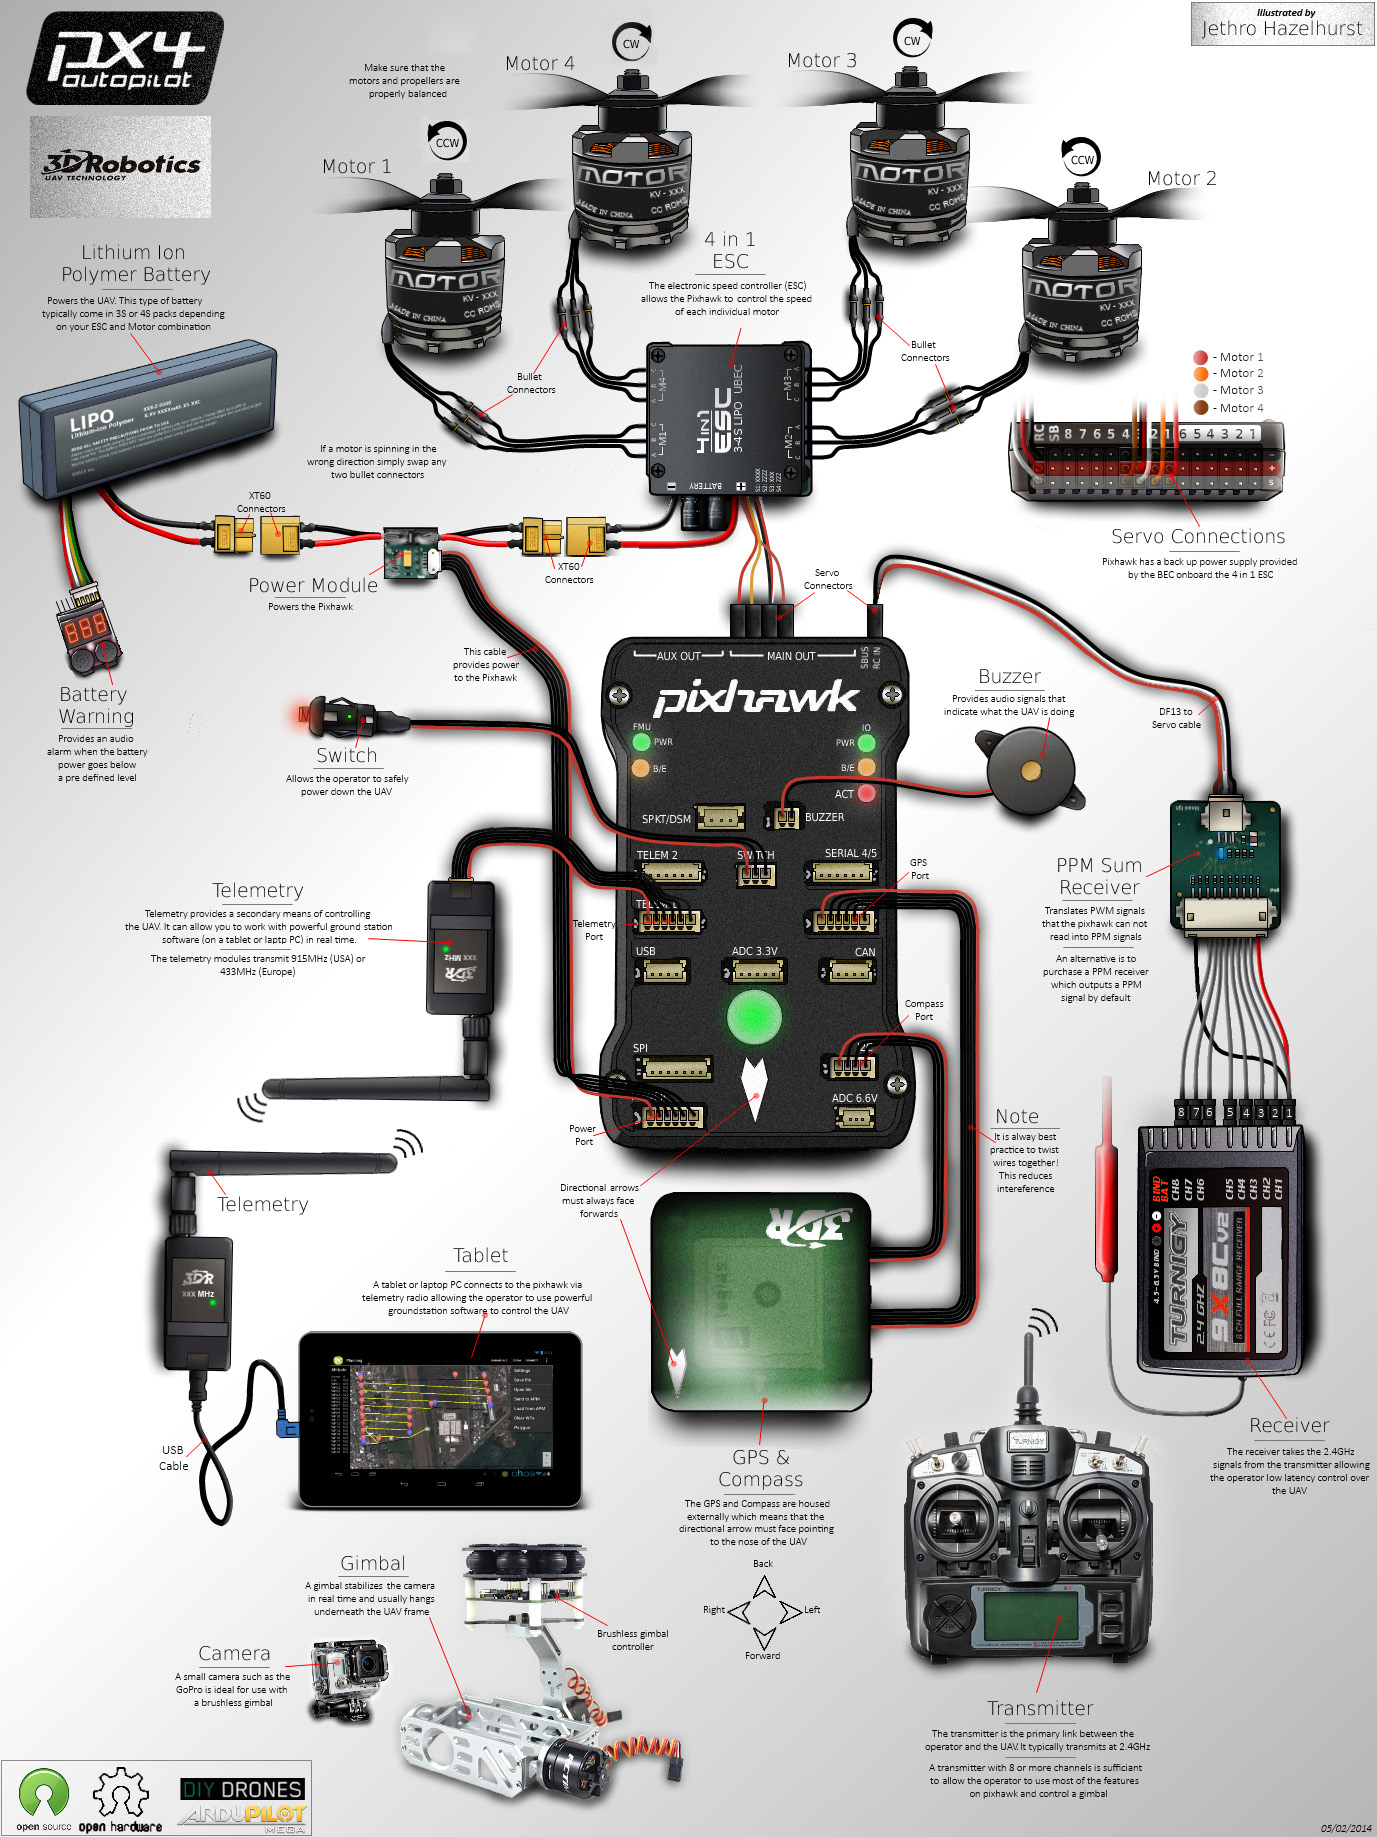
\includegraphics[scale=0.45]{pixhawk.jpg}
\end{center}

\paragraph{Power} 
\vspace{-3mm}
\ \\
\ \\
The 4 motors and flight controller will be powered by a 5200 mAh battery. This battery will power the drone for at least 15 min. The battery will be equipped with a battery monitor so that an alarm will go off when the battery power goes below a predefined level.  If this occurs, the drone will immediately perform a controlled landing at the nearest safe location.  Failure to deliver the package is preferable to crashing violently and damaging the drone's hardware.  The battery will be connected to the PTH08080W switching modulator that will divide power between the electric speed controller and the flight controller. Each motor will be connected to the 4 in 1 ESC.
\vspace{2mm}

\paragraph{Motors \& ESC}
\vspace{-3mm}
\ \\
\ \\
Our drone implementation will require four large drone motors.  The primary concern when choosing these motors is their thrust to weight ratio. A Q Brain 4-in-1 ESC will be used to control and regulate power to these motors. The device already has pre-installed motor leads terminated with 3.5mm bullet connectors and 4 signal leads to connect directly to the flight controller's ESC output ports. The input voltage required is between 7.4 and 14.8 volts. If the weight of the drone's components begins to hinder its ability to fly, the ESC should be one of the first devices slated for replacement.  The ESC weights 112g, making it one of the heaviest components, aside from the cargo compartment, that must be mounted on the drone.  The 4-in-1 ESC may be replaced with four inline ESCs which only weigh 10g each.  However, using these in-line ESCs will require a completely separate power distribution board. 

\paragraph{Flight Controller \& GPS}
\vspace{-3mm}
\ \\
\ \\
The flight controller selected is the PixHawk HKPilot32. The device contains the central processing components that will be used to control and monitor acceleration, air pressure, stability, speed, heading.  It also possesses ports for easily connectivity with the telemetry and GPS compass modules. The device has serial ports which allow for communication with another onboard computer such as an Raspberry Pi.

\ \\
The GPS is housed in a separate module that seamlessly connects to the flight controller. Inside the module is a Ubox LEA-6H GPS receiver and a HMC5883L digital compass.  

\paragraph{Frame}
\vspace{-3mm}
\ \\
\ \\
The AQ-600 is the quad copter frame selected for our design. The body is fabricated from carbon fiber to ensure light weight (400g in total) and durability. The rotor arms can fold in for easy storage/transport. The center of the body will act as a stable platform for attaching the flight controller, ESC, and various other components. This frame also possesses a protective shell to house all the components.  Due to expected modifications during our implementation process, this stock enclosure may not fit.  If so, the final design will instead possess a 3D printed enclosure to protect all electronics. The legs arc out slightly before connecting to parallel landing skids (like a helicopter).  The drone sits about 9 in. off the ground.  The large space between the drone and it's landing feet will permit the mounting of a large cargo compartment to house any and all packages.  The cargo compartment will either be fabricated using lightweight aluminum or it will be custom fabricated on a 3D printer.   

\paragraph{Telemetry/Radio Communication}
\vspace{-3mm}
\ \\
\ \\
The drone will house a telemetry system containing a 4G-LTE cellular data module and a GPS sensor. The telemetry module will be used to communicate with the server through a TCP/IP interface.  Alongside, the GPS sensor will be used for navigating from one location to another, while reporting its current location to an internal server.    

\ \\
The online web interface will send requests to the drone. These requests will contain information about a delivery, including a pickup location and destination address. The drone will be able to receive these requests and send status reports to the server indicating progress on the current delivery.  This progress data will be used by the online web interface to display information to the user, so that the package may be tracked in real time.  The continually updating information presented to the user will include the current location and projected course of the drone on a simple map, its current speed, and the ETA of the package based on the current course and speed.  An extension of this user interface containing more useful data (such as drone battery and other system statistics) will be provided to administrators/developers in order to assist in debugging any unexpected problems mid-flight should they occur.  

\paragraph{Proper Operation}
\vspace{-3mm}
\ \\
\ \\
When the drone receives a delivery request, it will fly to the designated starting location and wait for cargo to be loaded by a distributor.  The drone itself will possess a small button that the distributor may press to indicate that the payload was successfully loaded.  After a package has been loaded and the button has been pressed, the drone will immediately depart and journey to its destination. If, for any reason, the user wishes to change the package's delivery point, he or she may navigate to QUAC's online web interface and alter the destination's GPS coordinate.  After the user completes this operation, the server will signal the drone to navigate to a new location instead of its original destination. The drone will then promptly change course and travel to the new delivery point.

\subsection{Approach for Design Validation}

\section{Engineering Standards}

\subsection{Project Management}

\newpage
\subsection{Schedule of Tasks, Pert \& Gantt Charts}

\ \\
The Gantt and PERT charts provide a preliminary layout of the timeline and division of tasks of this project. The Gantt chart enumerates the breakdown of what each individual should be working on in a given week.  The tasks on the Gantt chart are color coded to indicate whom they are assigned to.  The length of the colored box on each row of the chart denotes the expected duration of each event.  

\ \\
The PERT chart offers a different view of the same tasks from the Gantt chart, but in a way that will allow us to evaluate the timeframe of individual tasks and how the relate to the critical path. The projected project length is 11 weeks and is expected to be complete around the $14^{th}$ of November. This will leave time for final testing and presentation before the end of the semester. Working as a team will allow us to concurrently schedule tasks and finish them in a timely manner. The design faces two main bottlenecks. Writing the proposal and all the associated research will require us to answer all design specific questions.  No one on the team has experience in drone construction.  As such, this research is time consuming and tedious.  Until research is complete, parts cannot be ordered.  Even after we completely determine the parts which will be required, we will be at the whim of distributors as to how quickly our parts are shipped.  Once parts arrive, we will progress by assembling the drone while simultaneously configuring the back end components.  Afterwards, a simple hardware/flight tests can be attempted followed by a full scale package delivery attempt. 

\begin{center}
    Figure \#\textbf{2}: Gantt Chart
\end{center}
\begin{center}
    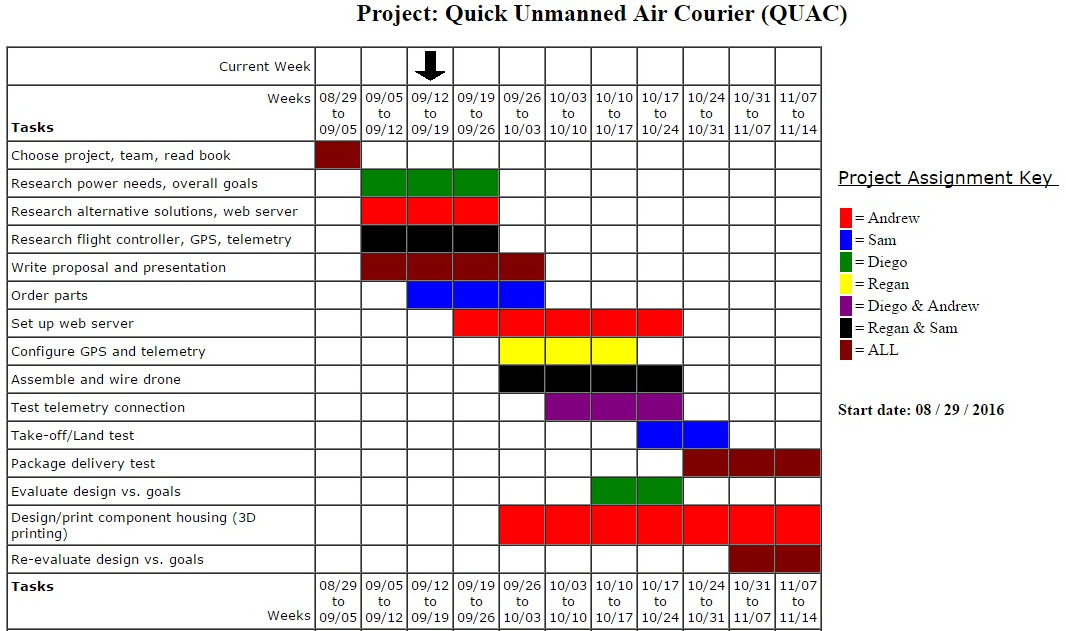
\includegraphics[scale=0.6]{gantt_chart.jpg}
\end{center}
\newpage
\noindent
\begin{center}
    Figure \#\textbf{3}: Pert Chart
\end{center}
\begin{center}
    \includegraphics[scale=0.30, angle=270]{PertChart.png}
\end{center}

\subsection{Economic Analysis}

\subsubsection{Economic Viability}

Initially, it seems that a drone delivery system would have limited applications.  The thought of a drone delivery network evokes visions of massive distributors, such as Amazon, who regularly sell and ship billions of dollars in products.  However, our team envisions a much larger market for our system.  Instead of restricting our solution to only large enterprises, we believe that it can be useful for any scale of business.  Large distributors can utilize massive networks of our drones to deliver their products.  In the same way, small companies, stores, and even restaurants can utilize a small number of drones (potentially networks as small as only one drone) running on the same type of server system to accommodate their needs.  

\ \\
Since one of the key design goals of our product is to cost less than employing a delivery driver, financial benefits should be evident to all interested parties.  Since a wide berth of enterprises stand to benefit, and our solution is scalable, we anticipate a large and continually growing market for our drone networks.  



\subsubsection{Sustainability}

The main component that our drone requires is the PixHawk flight controller.  It serves as a primary control system that manages and coordinates all other modules on the drone.  Everything from the electronic speed controller (which powers and regulates the motors) to the GPS and telemetry units can be accessed and managed through it.  The PixHawk is produced in a similar manner to ARM microprocessors.  A central company releases designs for the system and then any vendor may produce their own version/implementation.  As such, there are a large number of vendors for the PixHawk system.  Consequently, we do not anticipate any issues acquiring components on a large scale.  

\ \\
In the same way, the remaining components, such as motors, GPS module, and battery, are widely produced by a large number of corporations.  As such, there is limited risk of our project becoming dependent on a single producer.  

\ \\
Due to the mechanical nature of our product, we must anticipate that many parts will break or wear out in operation.  Most commonly, motors and batteries will need to be replaced.  However, these components are not expensive given that they should operate for reasonably long periods of time before wearing out.  The drone's frame and other electronics, the most expensive components, should not wear out quickly because they do not have any moving parts.  It is highly probable that the lifetime of those components will exceed the amount of time that it will take to replace them with new technology.   

\subsubsection{Manufacturability}

\ \\
Currently, the primary hindrance to our project is the FAA.  Existing regulations completely prohibit the use of unmanned aerial vehicles for commerce.  Such regulations stem from the inherent risks to personal safety and various ethical considerations (See Section 2.3 Design Constraints \& Feasibility).  In order to make our product ready for mass production, laws in the United States will need to be changed to allow drone commerce.  To do so, we, and others who wish to enter this industry, must prove to the government that our drone solutions are safe and can function without violating the publics' privacy.

\ \\
In general, moving parts are most vulnerable to variations in manufacturing.  Specifically, the motors in our design are rated to spin at a certain speed, $v$, for a certain input voltage, $V$.  Even though they are rated for a variety of (speed, voltage) pairs, every motor is slightly different.  Given this fact, it is easy to imagine a drone with four motors where 3 spin faster for a voltage $V$ than the fourth.  If this were the case, the afflicted drone would continually list towards the side with the weaker motor.  Thankfully, the effect is mitigated because the PixHawk is able to make corrections in motor voltage using a built in accelerometer.  Consequently, variations among motors will not be a significant concern.  

\ \\
In addition, we expect there to be marked variances in capacity and capability between different batteries, and even between different charges.  Such variances directly impact the operational range and time of our device.  In the worst case, we will assume that our system will only function with direct line of sight to the telemetry receiver and that the battery life will limit our operational time significantly.  Any optimizations that we make will be to increase flight time as much as possible.   

\ \\
Since our preliminary drone design will use telemetry instead of a full 4G connection, variations in battery strength will affect our operational range.  Our software will have to be specifically designed to attempt to avoid situations where signal is lost.  Unfortunately, this may come at the cost of reduced range.  Ideally, in a production system, our drones will be equipped with 4G modules which will communicate with nearby cell towers.  Such a system would not be afflicted as heavily with variations in signal connectivity.

\ \\
We are unable to predict our expected production yield due to insufficient knowledge of true customer demand and lack of any actual production facility.  However, given real resources, our drone could be manufactured quickly as it consists of a few modular off-the-shelf parts.  This modularity not only makes our design easy to build, but also it makes it easy to test.  Each component can be tested relatively independently of any others, making effective construction of drones easy.  

\ \\
As with many electronic devices, the disposal of our drones after their useful life has ended is a concern.  Batteries and printed circuit boards contain toxic chemicals which are capable of leeching into the environment.  Consequently, all of these parts must be recycled by the appropriate individuals.  

\ \\
In conclusion, we will be sure to design our system to always utilize components which comply with any and all FCC regulations regarding the operation and use of wireless devices.  


\subsection{Societal, Safety, \& Environmental Analysis}

Our drone system has the potential to modify an entire industry.  As such, it is possible that massive ramifications could result as a consequence of the technology that we develop.  Therefore, it is necessary to fully enumerate and consider the potential impacts of our solution, both positive and negative.  

\ \\
Our primary motivator in creating a UAV to deliver packages is to expedite the delivery process.  The current state of which is one of the only detractions from online shopping.  Consumers, especially those in America, are impatient and want to receive their newly purchased possessions immediately.  Even though online retailers are usually able to charge less for similar products sold in showroom stores, if one's need/want is great enough, the time to acquire the item outweighs any price differences.  Given that our solution can reduce the time of delivery from days to mere hours, this problem will no longer exist.  Shoppers will receive their goods in a timely manner without ever having to leave the comfort of their own homes.  

\ \\
However, as is always the case, there is no such thing as a free lunch.  Where there is a positive, there must also exist a negative.  With delivery time reduced, traditional storefronts will no longer have any benefit over online retailers.  Consequently, the action of bypassing retail will most likely put many shops completely out of business.  The same could even potentially be said of large shipping empires.  Surprisingly, a large chunk of the deliveries that major delivery corporations handle are small items from bulk distributors such as Amazon.  Delivering packages via drone from one's own distribution center completely bypasses any need for UPS or FedEx, potentially hurting their business and profits significantly.

\ \\
Each closure means loss of jobs and potentially even ruined livelihoods.  One could say that this happens with every new technology, but with a potential impact this broad, it must be considered.  If the loss of jobs as a result of our solution ends up being extremely severe, it could potentially be mitigated by retraining store owners and employees to work with our products as drone maintainers or system operators.  However, there is no way to know how widespread the impact will be until a rapid delivery system such as ours is actually implemented.  

\ \\
In addition to financial concerns, our team must consider the physical safety of our designs.  Drones, especially those carrying packages, are heavy.  If something were to go wrong mid flight and the drone goes down, what happens?  Since there is no human pilot at the helm, how will it know to avoid living beings and structures?  Saying that nothing will never go wrong is a logical fallacy, instead we must do our best to mitigate and prepare for potential incidents.  Specifically, our design will be equipped with sensors to detect nearby objects in an attempt to avoid simple collisions in flight.  A more capable prototype could also be equipped with a camera in order to sense the environment around it and make more informed avoidance decisions.  Other changes could come in the form of policy instead of hardware.  Obviously, it would be disastrous if a drone were to cause a car accident by crash landing on a crowded roadway.  The routing algorithm for our drone can be programmed to avoid traversing major roadways as much as absolutely possible.  

\ \\
Along with avoiding accidents involving living beings, our drone should account for privacy concerns.  One of the primary reasons for restrictions on drones today is that people are afraid that their privacy and property will be invaded by multitudes of small flying objects.  As such, our current prototype will be implemented without using a camera in order to eliminate the possibility of any unauthorized photography.  Future designs which operate in residential environments will also need to avoid private property unless express permission is provided by the landowner (i.e. if someone orders something, that is implicitly giving the drone permission to enter their estate.  

\ \\
Finally, we expect a positive impact on the environment as a result of implementing our drone.  Current delivery trucks run on either gasoline or diesel which are significant sources of pollution in our world today.  Our UAVs run on electricity.  Not only is an electric system much more efficient than a gasoline engine, but also, the electricity that powers our drones could be derived expressly from renewable sources.  

\ \\
The list of considerations and concerns is lengthy.  Therefore, being considerate of them is paramount for our project.  Failure to adapt our design to social, physical, and ethical concerns could turn a novel project into an utter failure. 


\subsection{Itemized Budget}

\begin{displaymath}
{\setstretch{1.5}
    \begin{array}{cc}
        \hline
            \textbf{Item}\phantom{aaaaaaaaaaaaaaaaaaaaaaaaaaaaaaaaaaaaaaaaaaaaaaaaaaaaaa} & \textbf{Expected Cost} \\
        \hline
            \text{(1) PixHawk Flight Controller Kit}\phantom{aaaaaaaaaaaaaaaaaaaaaaaaaaaaaa} & \text{\$190.82} \\
            \text{(4) Drone Motors + Propellers}\phantom{aaaaaaaaaaaaaaaaaaaaaaaaaaaaaaaa} & \text{\$117.72} \\
            \text{(1) Q Brain 4-in-1 Electronic Speed Controller}\phantom{aaaaaaaaaaaaaaaaaaaa} & \text{\$31.81}\phantom{a.} \\
            \text{(1) Multistar 3S 5200 mAh Drone Battery}\phantom{aaaaaaaaaaaaaaaaaaaaaaa.} & \text{\$41.74}\phantom{a.} \\
            \text{(1) AQ-600 Carbon Fiber Quadcopter Frame}\phantom{aaaaaaaaaaaaaaaaaaaaa.} & \text{\$56.68}\phantom{a.} \\
            \text{Miscellaneous Components and Wires}\phantom{aaaaaaaaaaaaaaaaaaaaaaaaaaa.} & \text{N/A} \\
            \text{Rapid Prototyping for Enclosure \& Cargo Compartment}\phantom{aaaaaaaaaaaa} & \text{\$0.00}\phantom{aa.} \\
        \hline
        \hline
            \textbf{Total Cost}\phantom{aaaaaaaaaaaaaaaaaaaaaaaaaaaaaaaaaaaaaaaaaaaaaaaaa.} & \text{\$316.61}\phantom{..} \\
        \hline
    \end{array}
}
\end{displaymath}

\section{References}

\nocite{*}
\renewcommand\refname{\vskip -1cm}
\bibliographystyle{IEEEtran}
\bibliography{bibliography}


\section{Appendices}

\subsection{Product Datasheets}

All product datasheets are attached at the end of this report.  

\subsection{Bios \& CVs}

\ \\
{\large \textbf{Andrew Kirfman}} is a student at Texas A\&M University.  He is currently in his final year of working to earn his undergraduate degree in Computer Engineering, planning to graduate in May of 2017.  

\ \\
Andrew's parents, John \& Kim, both graduated from A\&M in 1989.  John earned a degree in Electrical Engineering, and Kim earned a degree in Education and Curriculum Instruction.  Andrew was home schooled by his mother throughout his entire K - 12th grade education.  Being home schooled allowed Andrew the freedom to explore a multitude of subjects not normally available to most students.  Specifically, the ability to use school hours for learning about computers and programming (both activities encouraged by Andrew's father).  

\ \\
Throughout high school, Andrew took dual credit classes at a local community college.  After taking his first programming class (An intro to C++ programming course), he was recommended, by his computer science instructor, for a job with the college's computer support department.  A job that he held throughout the rest of high school. 

\ \\
After completing high school, Andrew begin taking courses full time at A\&M.  He is fascinated by a wide variety of subjects, but has specifically enjoyed his courses in operating systems, digital logic, VLSI design, and low level programming.  

\ \\
During the summer of 2015, Andrew interned with Tektronix Communications in their platform development group.  There, he worked writing code and applications for a custom Linux distribution based off of Debian.  In doing so, he trained himself to be fluent in Python, Bash, and many other linux utilities and tools.  During the other two summers (2014 and 2016), Andrew spent his time taking courses in order to fulfil degree requirements at A\&M.  

\ \\
After the conclusion of his studies at A\&M, Andrew hopes to intern somewhere in the Dallas area doing low level software engineering.  In the fall of 2017, he intends to enter graduate school in order to earn his masters, and eventually PhD, in either Computer Engineering or Computer Science.  

\ \\
{\large \textbf{Diego Oliveros}} is a senior at Texas A\&M University, majoring in Computer Engineering in the Computer Science track in December 2016. Diego's focus is software development. While he has learned most programming languages on his own, his work experience and education has helped in building his character, social skills, work ethic, and project management skills.

\ \\
Starting on January of 2016, Diego joined Amazon Business as a Junior Developer. He has been working part-time remotely as a software developer in the spring and fall, and full-time on-site over the summer. He is an active member of the Business to Business Accounts team, working using Java, Spring, Amazon Web Services, XML Configurations, Ajax, and NoSQL database management to help Amazon customers build their businesses.

\ \\
In the summer of 2015, Diego had an internship with Cisco in San Jose, California. He worked using Python and internal Cisco tools to build a system which automated the creation of test files used to test different calls and handovers for major Cisco customers.

\ \\
Previous work experience include working as a Freelancer in his brother's company, Kinui. He worked using HTML, CSS, Ajax, PHP, MySQL database management, jQuery, Javascript, and some Content Management Systems, including Drupal, Joomla, and Prestashop.

\ \\
After graduation, Diego plans to work fully remotely as a Software Developer.

\ \\
{\large \textbf{Regan Vecera}} was born and raised in the small town of La Grange, Texas. His natural proclivity for math and science led him to computers from an early age. His interest was piqued when he took his first computer science course in 10th grade and started learning Java. Also while at La Grange H.S. Regan explored many other interests including video game design, audio/video production, and home/ small business networking and competed in many academic competitions including number sense, mathematics, computer science, and science. His senior year was filled with AP and dual credit courses and culminated with to obtainment of valedictorian.  

\ \\
Upon graduating, Regan was immediately accepted into the Computer Engineering department at Texas A\&M, along with the University Honors program. He entered with 33 hours. His first year, Regan lived on campus which made it easy for him to participate in the Texas A\&M Computing Society (TACS), intra-mural sand volleyball, and various honors engagements.  While at Texas A\&M, Regan continued his course of study in engineering with no intentions of deviating. 

\ \\
Between his freshman and sophomore years, Regan worked as an intern for True Protection LLC. The internship was a 14 week summer program in Plymouth, MN. Regan, along with 15 other interns, were advertising directors responsible for cold calling door-to-door to solicit home security, home automation, and life safety technology. The experience was not of technical significance, but was more about learning how to work on a team, how to control your emotions, and how to communicate with word choice, tonality, and body language.

\ \\    
The summer between sophomore and junior year, Regan traveled to Brazil to take two courses in electrical engineering and experience the atmosphere of a foreign country. There he learned the basics of linear control systems and Portuguese. 

\ \\    
The first two and a half years consisted mainly of taking the lower level prerequisites and university core curriculum. Once admitted to the upper level courses, Regan focused his skills on design and analysis of algorithms, robotics/embedded systems, and a math minor. His current interests are in the areas of cyber security and artificial intelligence. Upon graduating in Dec. 2016, Regan intends to find a full time job as a penetration tester. After some time industry to acquire knowledge, capital, and connections, Vecera has his sights set on becoming an entrepreneur.  

\ \\
{\large \textbf{Sam Gwydir}} is a senior at Texas A\&M University. He will obtain his Bachelor of Science degree in Computer Engineering with a Computer Science focus in May 2017. Sam's priority in going to university was learning those software and hardware topics that aren't easy to learn without expert mentorship, i.e. a professor and course.

\ \\
Mr. Gwydir is an active participant in the FreeBSD, Linux and larger open source community. He has spent many semesters tutoring programming, in particular C++. He also spent one semester converting Dr. Bassichis' Don't Panic from classic TeX to DocTeX templates in modern LaTeX. In addition he was part of Aggie Toastmasters for 2 years, spending his second year as social chair, helping to recruit new students for the club. Mr. Gwydir has also contributed to several open source projects including but not limited to: iTerm2, Emacs, Spacemacs, and the FreeBSD operating system.

\ \\
Mr. Gwydir has interned with Groupon in Palo Alto, California for the summer of 2016 and will remained working for them part time throughout the year. That summer he joined the Systems Engineering team managing the Global Database Systems (GDS) department's database hosts. These hosts all run FreeBSD and it is his responsibility to document, test and improve the design behind Groupon's Databases as a Service (DaaS) project. Of particular importance were his benchmarks relating to MySQL and ZFS configurations.

\ \\
After his graduation in May 2017, Mr. Gwydir will begin his career as a Computer Engineer.




\end{document}
